\section{LLM Serving and Scheduling}
\label{sec:bg}

\subsection{Background: Scheduling LLM requests in a Cluster}
\label{sec:llm-scheduling}

\begin{figure}[!t]
        \vspace{2mm}
        \begin{minipage}{1\linewidth}
        \centering
        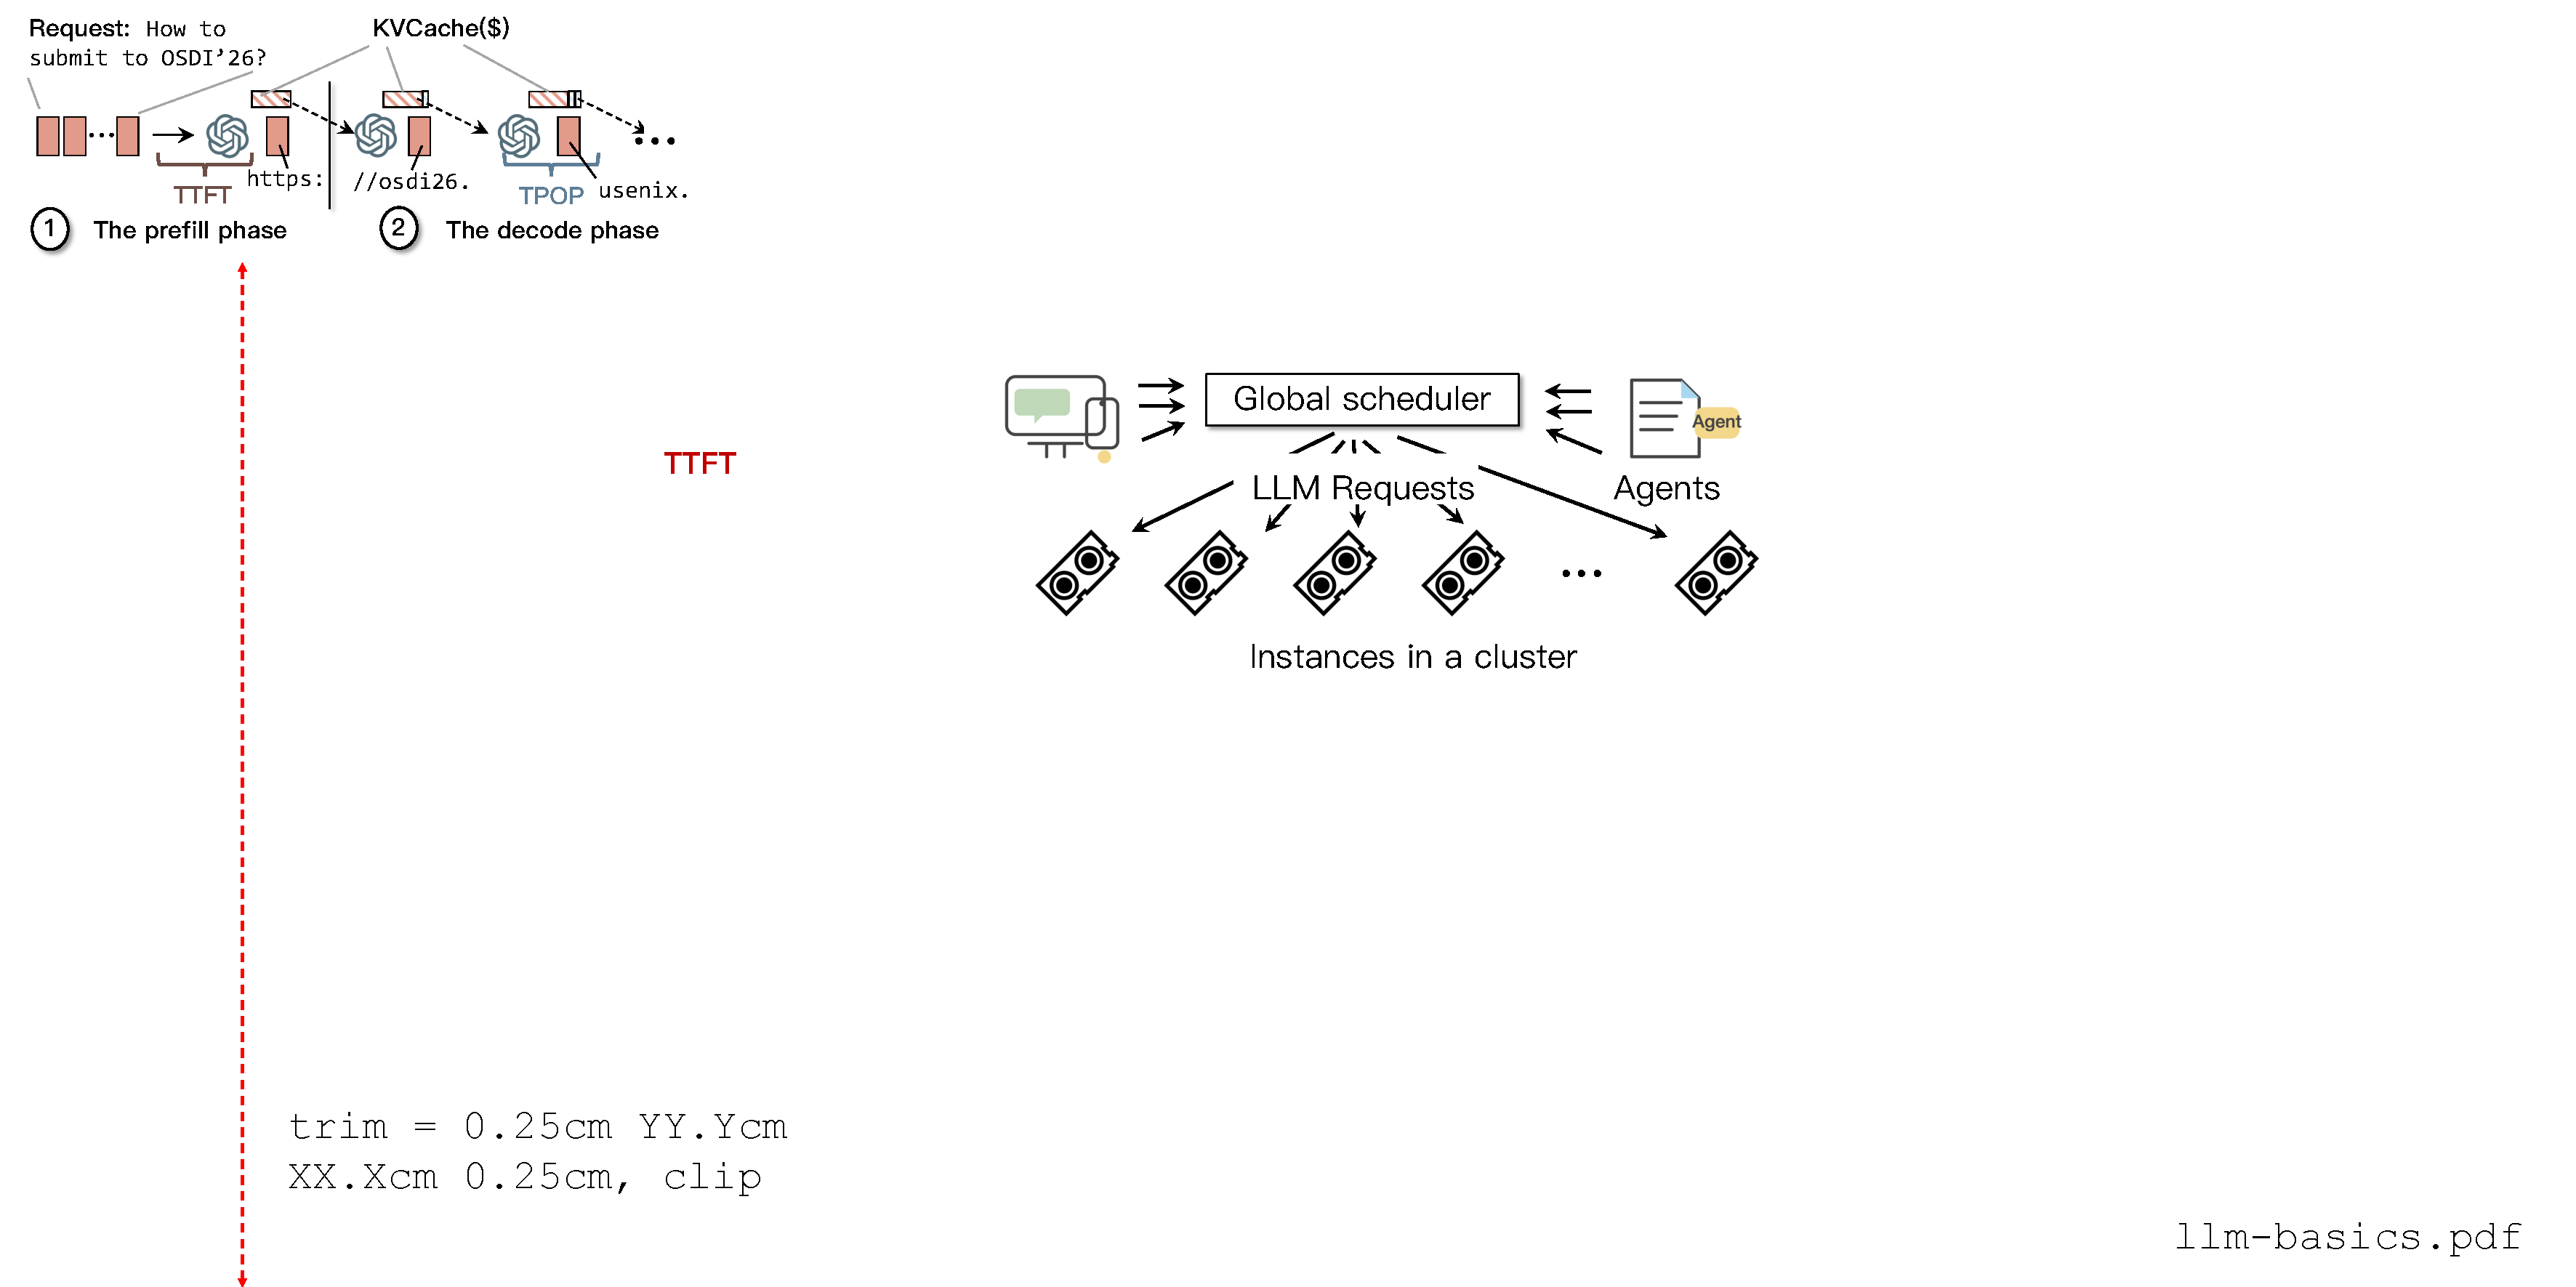
\includegraphics[width=0.95\linewidth, trim=0.25cm 23.92cm 43cm 0.25cm, clip]{figs/llm-basics.pdf}
        \end{minipage} \\[2pt]
        \begin{minipage}{1\linewidth}
        \caption{\small{%
            An illustration of generating output tokens 
            using an LLM and the two performance metrics: 
            time to first token (TTFT) and time per output token (TPOT).
        }}
        \label{fig:llm-basics}
        \end{minipage} \\[-0pt]
        \end{figure}


\nospacestitle{Serving requests with an LLM ({\fig{fig:llm-basics}}).   \,}
LLMs generate tokens in an auto-regressive manner
through two steps:
\ding{192}: In the \emph{prefill} phase, the input tokens are fed into the model,
and the model processes these tokens to
produce the first output token.
The LLM then enters the \emph{decode} phase (\ding{193}) to generate the subsequent tokens one-by-one.
Each generation requires the context of all previously generated tokens and the input tokens.
To accelerate generation,
the \emph{processed context} is materialized as tensors stored in GPU memory, typically
termed \emph{key-value cache} ({\kvcache}).
As a result, the computation in the decode phase is significantly smaller
than that in the prefill phase because no input token {\kvcache} needs to be generated.

From an LLM service provider's perspective, two key performance metrics related to the 
serving quality are:
\emph{time-to-first-token (TTFT)} and \emph{time-per-output-token (TPOT)}.
TTFT is important because it directly determines the LLM service's responsiveness to user requests,
while TPOT not only affects the subsequent responsiveness
but also the overall request completion time. 

\begin{figure}[!t]
        \hspace{3mm}
        \begin{minipage}{1\linewidth}
%        \centering
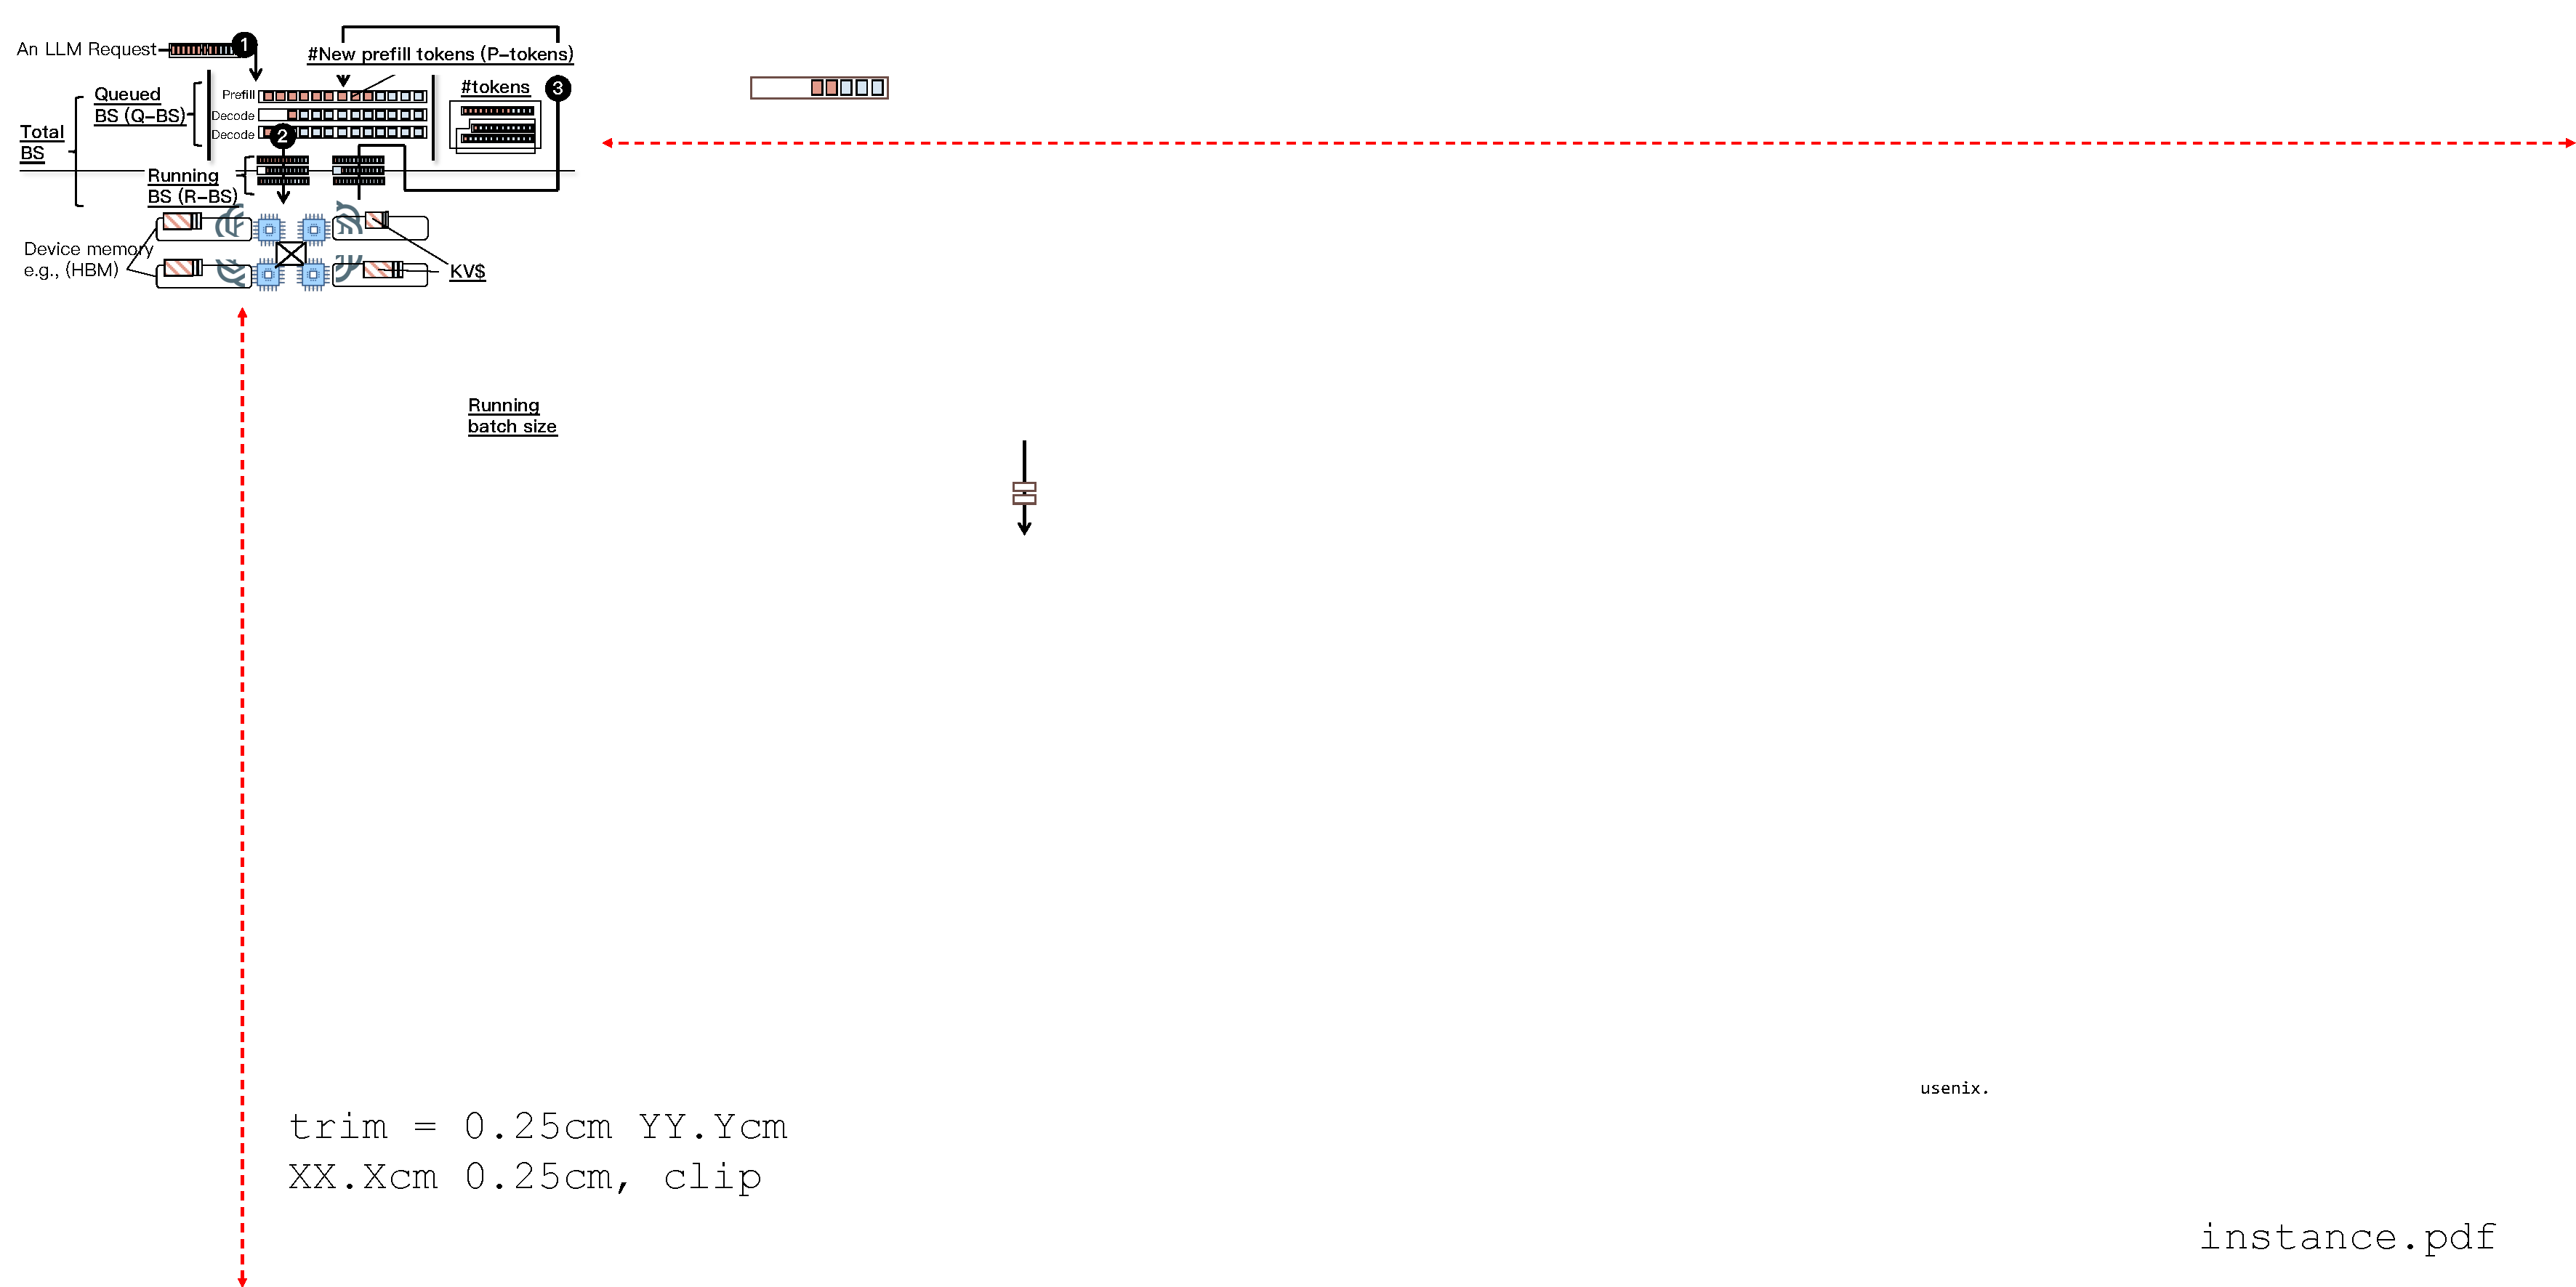
\includegraphics[width=0.92\linewidth, trim=0.25cm 22.9cm 46cm 0.25cm, clip]{figs/instance.pdf}
        \end{minipage} \\[4pt]
        \begin{minipage}{1\linewidth}
        \caption{\small{%
            The system view of how an LLM serving instance serves
            requests and some direct system \metric{indicators}
            that can be collected by the global scheduler. % (described in \textsection{\ref{sec:sys-metrics-llm-scheduling}}).
%            \textbf{\uline{TPS}} is the abbreviation for \uline{t}okens \uline{p}er \uline{s}econd. 
            The detailed meaning of each indicator will be described upon the first usage. 
            \textbf{BS} is the abbreviation for \uline{b}atch \uline{s}ize.
        }}
        \label{fig:llm-instance}
        \end{minipage} \\[5pt]
        \end{figure}


\stitle{Serving instance and {\kvcache} cache ({\fig{fig:llm-instance}}). \,}
In an LLM serving system, an instance is the minimum unit that serves requests and hosts one complete copy of the LLM parameters.
The instance can contain multiple GPUs if the LLM is too large to fit into a single GPU's memory.
Regardless of single-or-multiple GPU instances,
the overall serving flow is the same:
when it receives a request,
the request is pushed into a queue containing requests (either prefill or decode) waiting to be executed
on this instance (\ding{182}).
Once the GPU(s) become available, all queued requests are formed into a \emph{batch},
and the batch is executed on GPU(s) efficiently with 
\emph{chunked prefill}~\cite{298679} (\ding{183}). 
After the execution,
the instance examines whether the current requests need further decoding;
if so, the requests are re-enqueued (\ding{184}).

One notable feature is that the serving is \emph{stateful}: the request's {\kvcache}
is retained in GPU or CPU memory even after the request finishes its generation ({\kvcache} cache~\cite{305212,298501,10.5555/3768039.3768067}).
The benefit is that 
if a future request is routed to an instance and 
there is a prefix match with a previously cached {\kvcache},
the instance can skip the computation for the matched prefix tokens
and thus significantly reduce the computation cost.
In our example in {\fig{fig:llm-instance}}, tokens that are colored blue can skip the computation
if they have a {\kvcache} hit.
%For requests in the decode phase, all tokens except the last one have {\kvcache} hits.

\begin{figure}[!t]
%        \hspace{-2mm}
        \begin{minipage}{1\linewidth}
        \centering
        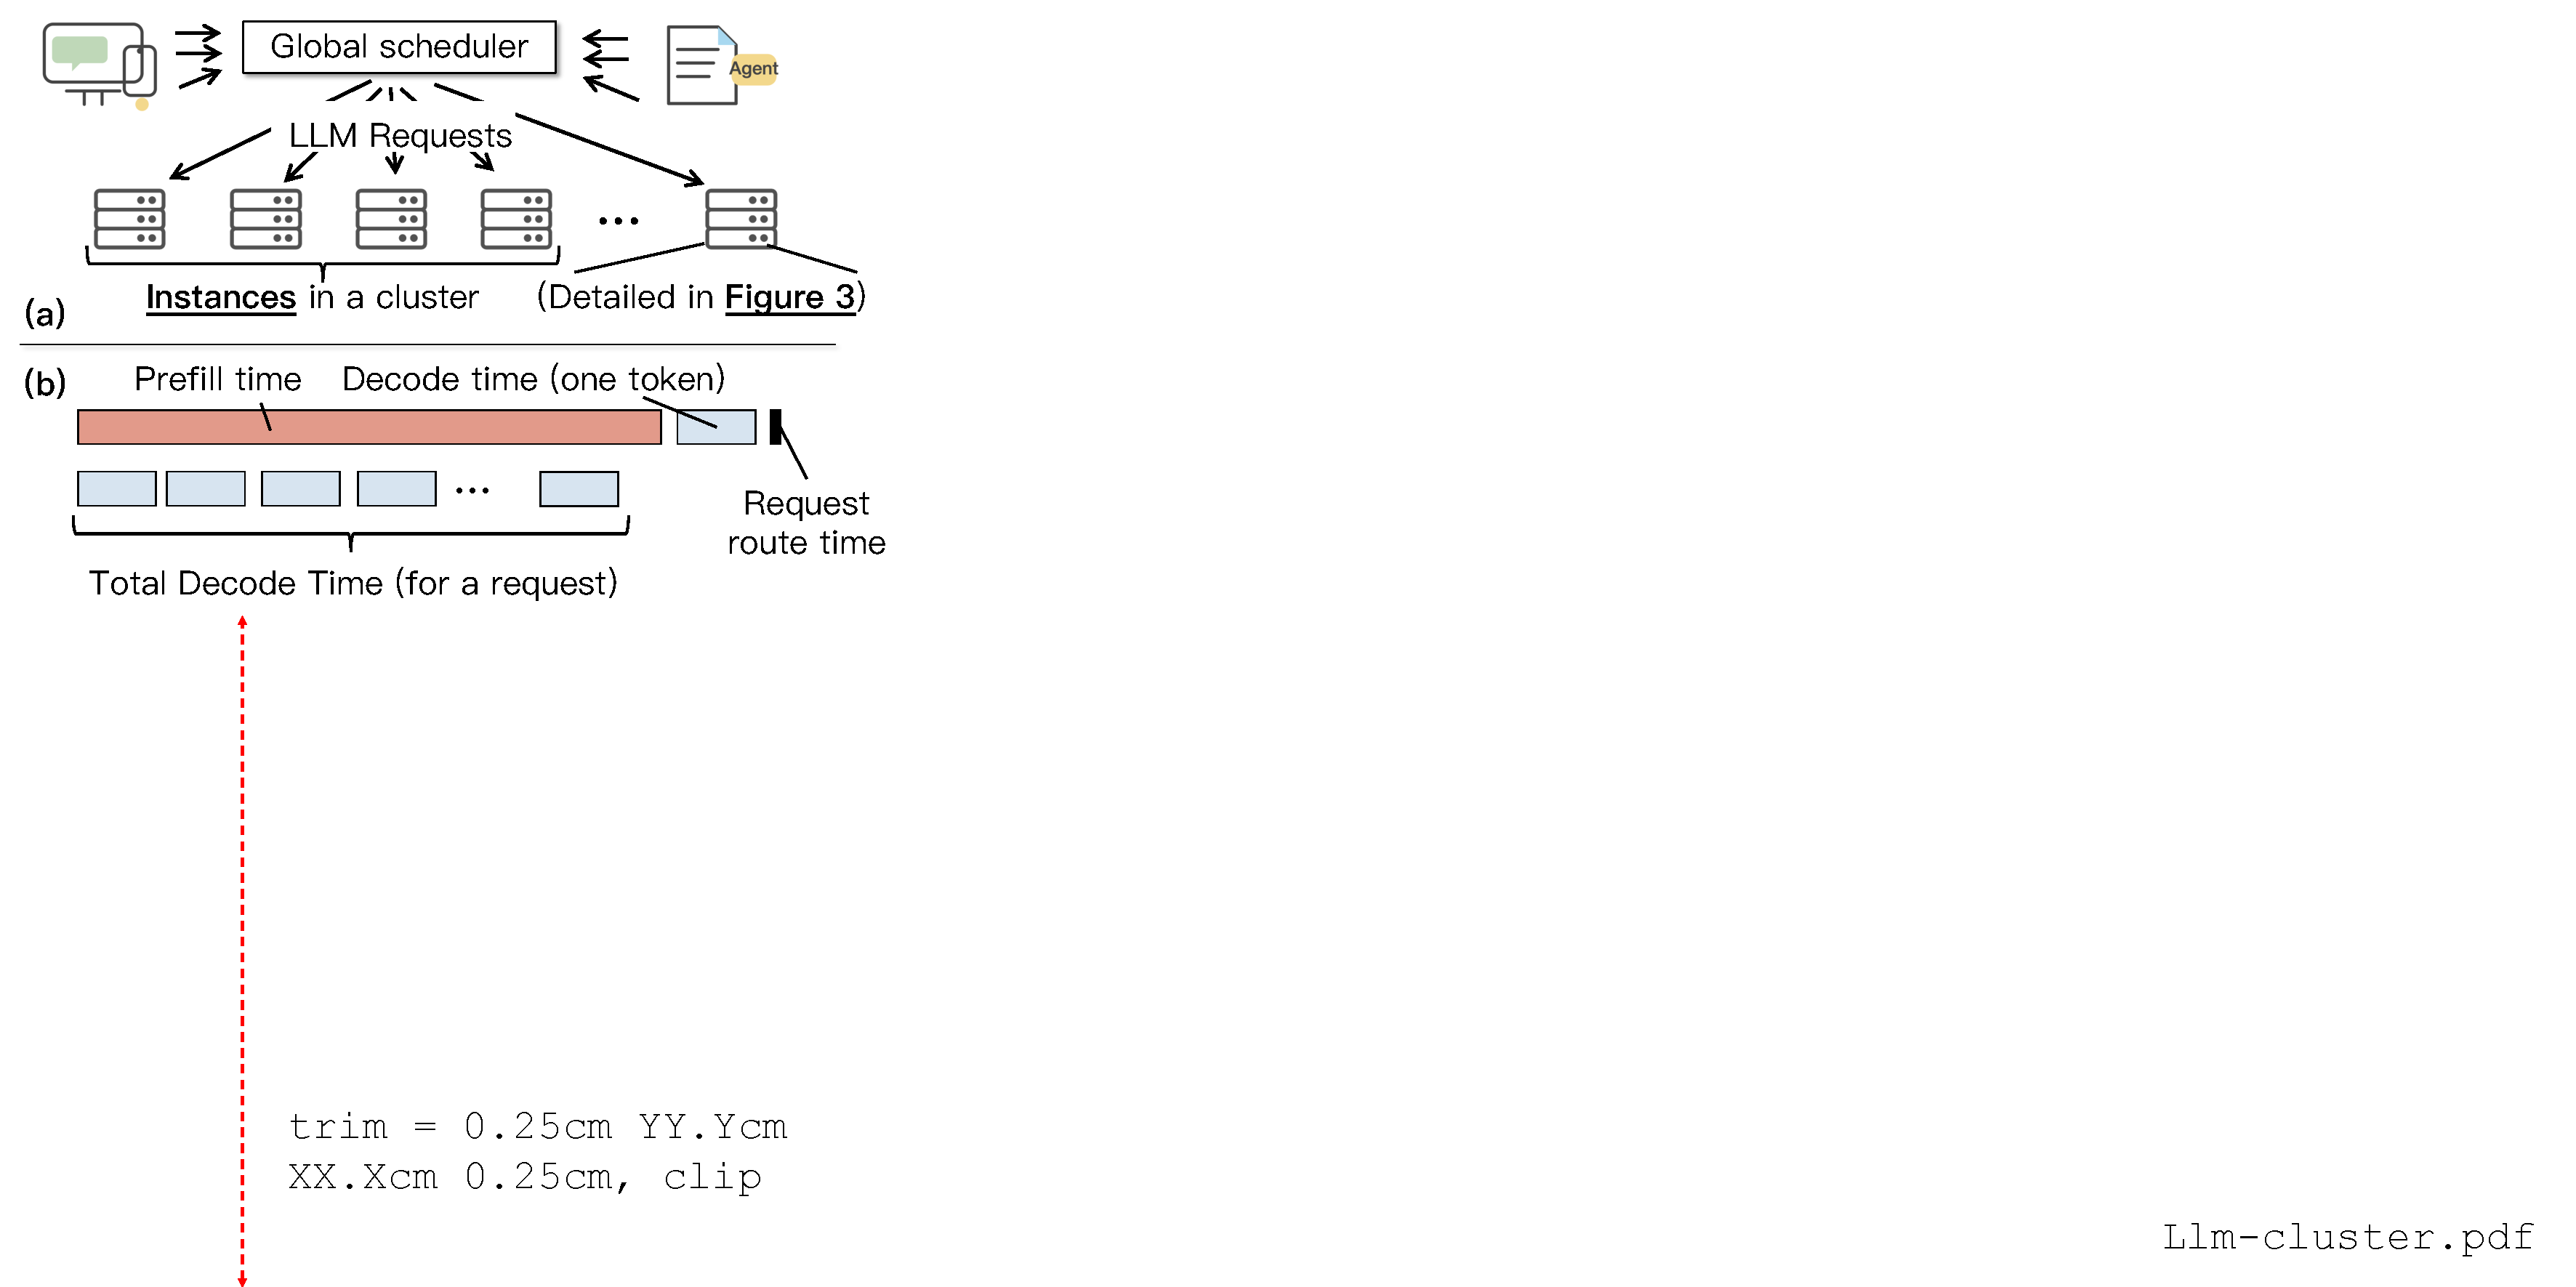
\includegraphics[width=0.85\linewidth, trim=0.25cm 15.7cm 39.65cm 0.25cm, clip]{figs/llm-cluster.pdf}
        \end{minipage} \\[4pt]
        \begin{minipage}{1\linewidth}
        \caption{\small{%
        (a) System view of a cluster LLM serving system,
        and
        (b) comparison of per-request serving time and routing cost.
        }}
        \label{fig:setup}
        \end{minipage} \\[-10pt]
        \end{figure}

\stitle{Request scheduling in a cluster ({\fig{fig:setup}}). \,}
To handle large volumes of requests,
LLM service providers typically deploy clusters of instances to serve a model,
where each cluster has a dedicated \emph{global scheduler} to route requests to the instances managed by it,
as shown in (a).
The scheduler executes a \emph{scheduling policy} to determine the destination instance for each request,
and this policy is our focus.
Note that the provider may deploy multiple clusters for the same model to enhance reliability and geo-affinity,
and routing requests between clusters is out of the scope of this paper.
%\highlight{Multiple clusters are required to enhance reliability and geo-affinity, 
%yet routing between instances is out of the scope of this paper}.

At a high level, all existing scheduling policies can be viewed as a three-step process:
The router first (optionally) \emph{filters} out some instances,
then \emph{scores} them according to a preference order,
and finally routes the request to the best-scoring instance.
The score is based on the indicators collected from each instance,
and we will describe them in detail in our analysis (\textsection{\ref{sec:principles}}).

\iffalse
\begin{figure}[!t]
%        \hspace{-2mm}
        \begin{minipage}{1\linewidth}
        \centering
        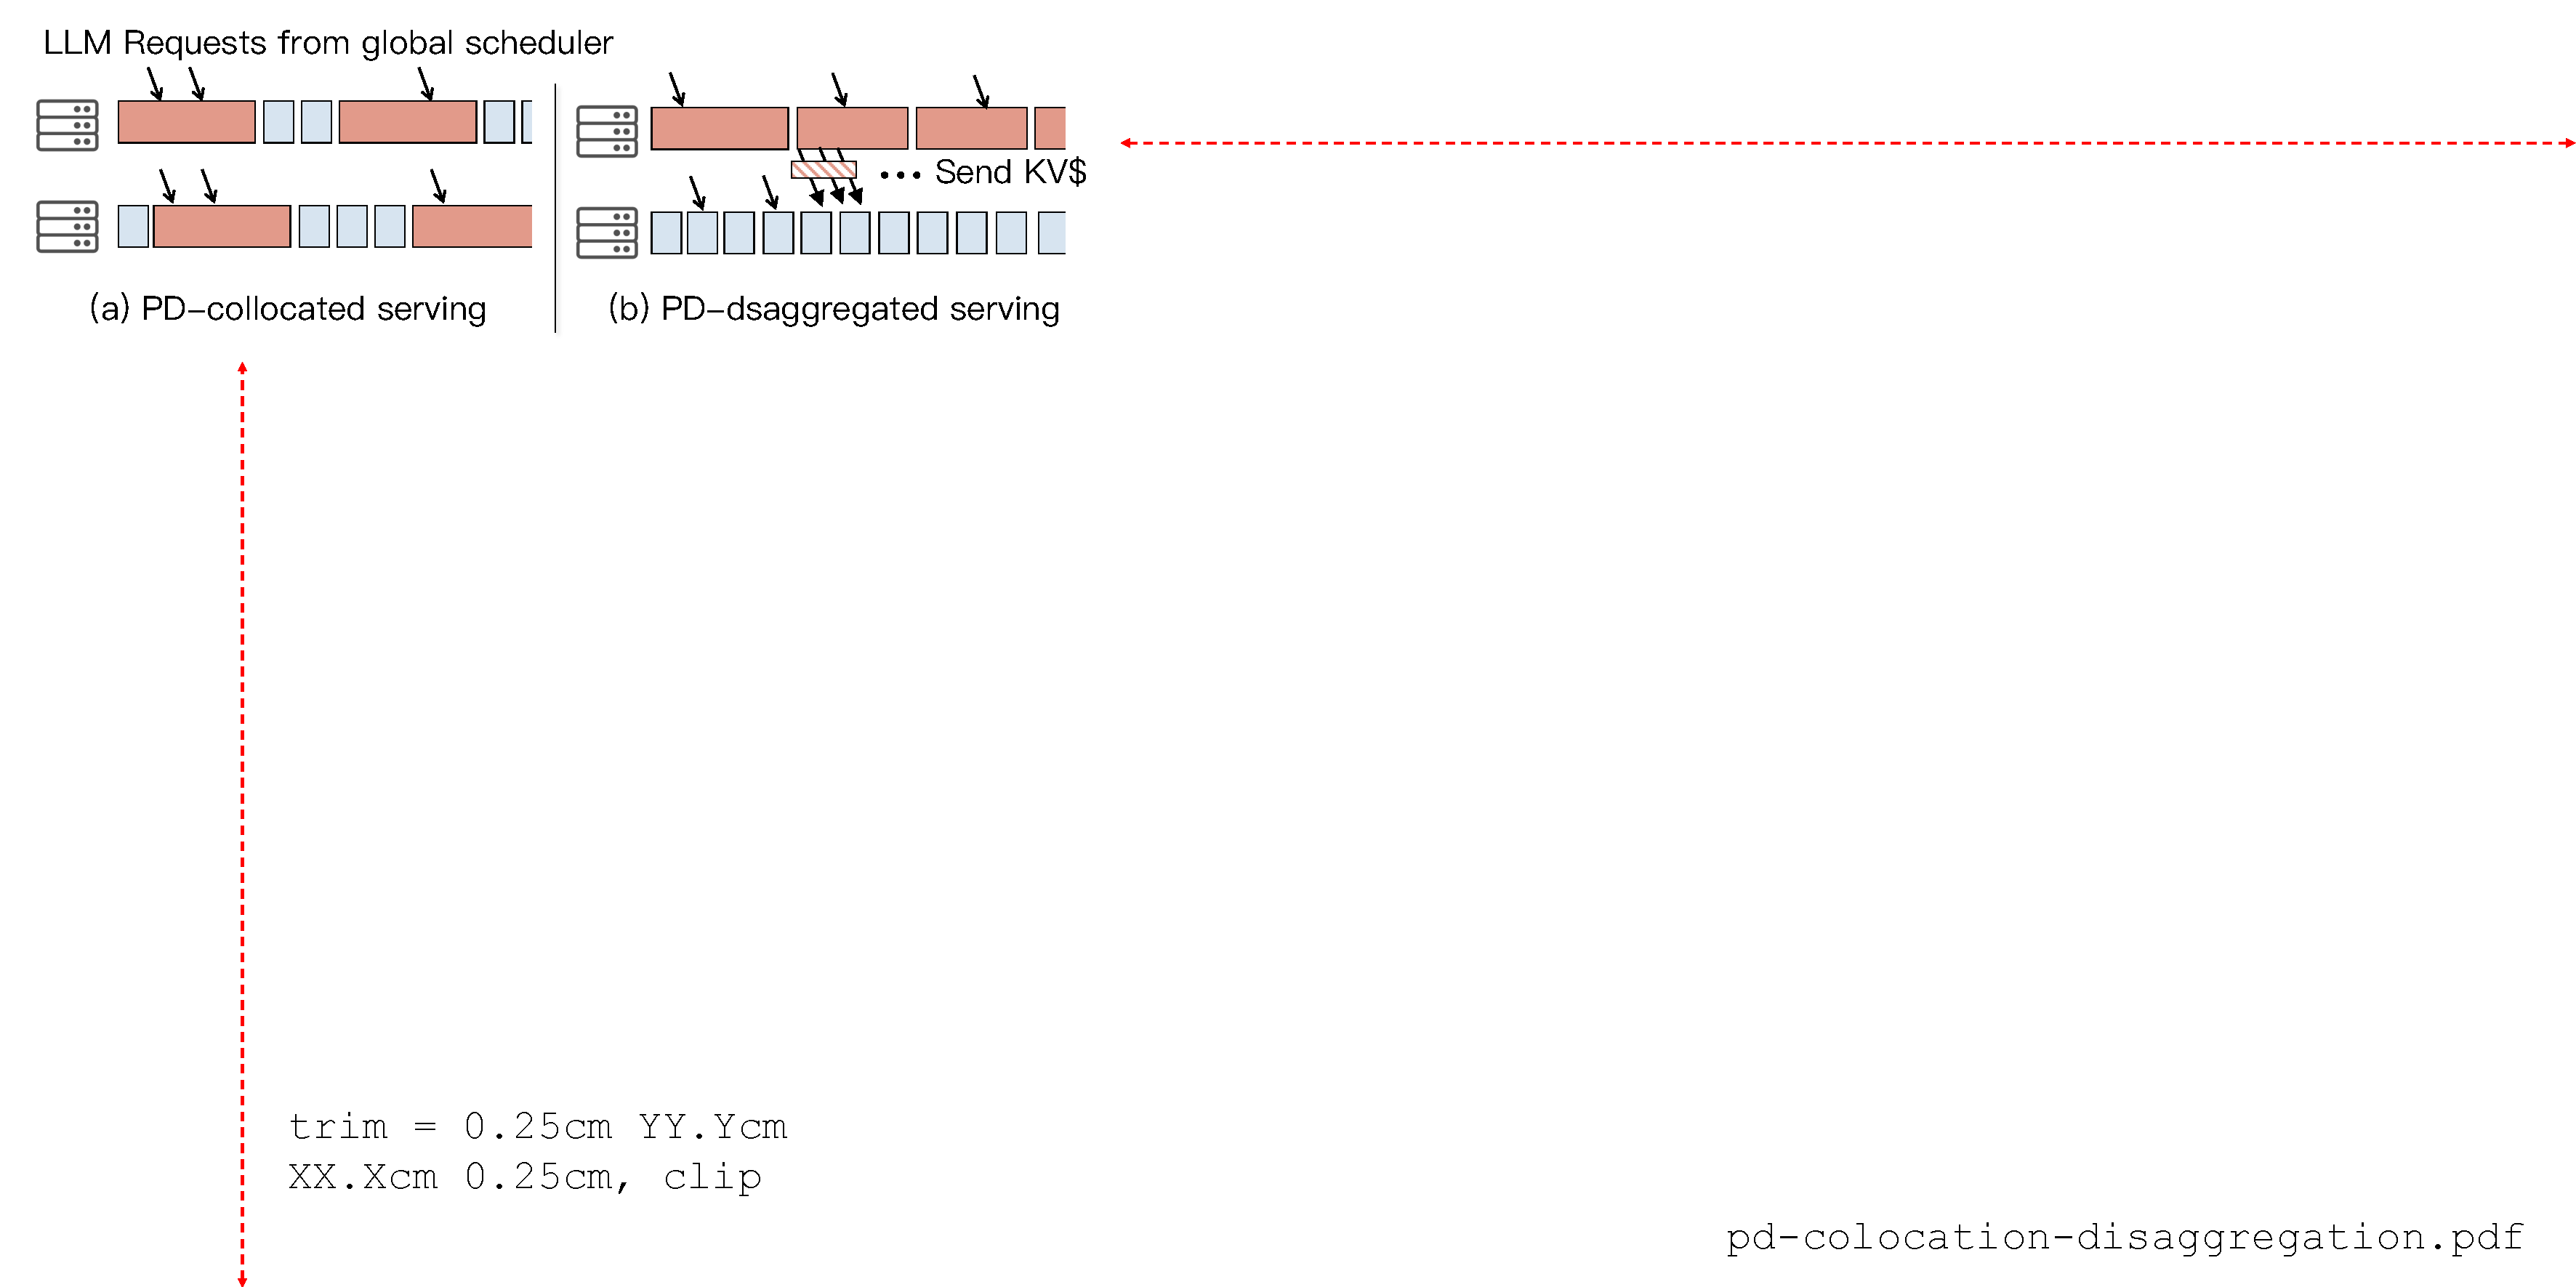
\includegraphics[width=0.99\linewidth, trim=0.25cm 21.6cm 33.95cm 0.25cm, clip]{figs/pd-colocation-disaggregation.pdf}
        \end{minipage} \\[0pt]
        \begin{minipage}{1\linewidth}
        \caption{\small{%
        A comparison of (a) request scheduling in PD-colocated serving and 
        (b) PD-disaggregated serving.
        }}
        \label{fig:pd-colocation-disaggregation}
        \end{minipage} \\[-20pt]
        \end{figure}


\stitle{PD-colocation and PD disaggregation ({\fig{fig:pd-colocation-disaggregation}}). \, }        
Finally, since the prefill and decode phases exhibit different execution patterns,
there exist two deployment choices: PD-colocated (a) and disaggregated (b).
In colocated serving, the execution flow on an instance is exactly the same
as we have described above.
On the other hand, in disaggregated serving,
each instance serves either prefill or decode, but not both.
As a result, the global scheduler needs to determine both the routing of prefill and decode instances
for each request,
and once the prefill is done, the {\kvcache} needs to be transferred to the decode instance. 
In this paper, we assume that the scheduler determines the instances simultaneously---the de facto
implementation in academia and industry~\cite{}, because such a design \TODO{DY: add refs}
could enable accelerated {\kvcache} transfer using layer-by-layer early transmission~\cite{DBLP:conf/isca/PatelCZSGMB24}.

\highlight{Both deployments have pros and cons so they are both deployed in {\company}. 
PD-colocated serving clusters are easier to maintain (no instance role management)
and do not rely on fast networking between instances for transferring {\kvcache}.
In comparison, PD-disaggregated serving provides effective performance isolation
between prefill and decode requests.}.
\fi

\iffalse
\subsection{Direct Indicators for LLM Scheduling}
\label{sec:sys-metrics-llm-scheduling}


\noindent
To the best of our knowledge, all existing policies
leverages numeric indicators collected at each instance as hints to make scheduling decisions.
The indicators that can be directly collected (and some simple variants) 
are summarized in {\fig{fig:llm-instance}} and described as follows:  \\[-10pt]
\begin{itemize}[leftmargin=*,leftmargin=10pt,itemindent=0pt]
    \item \metric{Batch size (BS)} is the number of unfinished requests 
        on each instance. 
        The unfinished requests can be further categorized into two types:
        \metric{Running BS (R-BS)} refers to the number of requests being executed on GPU(s),
        and \metric{Queued BS (Q-BS)} refers to the number of requests waiting to be executed.
        The requests can be queued because when a request is routed to an instance,
        the instance may be busy processing current batch and 
        the execution time of a batch is several
        orders of magnitude higher than the routing time (see {\fig{fig:setup}} (b)).
        \\[-5pt]

        \item \metric{\kvcache hit} is the hit ratio when the router decides to execute
        the request on a given instance. Note that computing the ratio is highly efficient
        because we only need to compare the request's prefix hash with the instance {\kvcache}'s hashes.

    \item \metric{\# Tokens} records how many tokens are running on the instance,
        including both the number of tokens waiting to be prefilling
        and the context tokens for decode requests.
        The token number is important because both the prefill and decode time is proportional
        to the number of tokens~\cite{DBLP:conf/osdi/ZhongLCHZL0024,DBLP:conf/osdi/ZhuGZZZGX0KLWWK25}.
%        so using R-BS and Q-BS alone is insufficient to estimate the load on an instance.
        Here, we explicitly distinguish between the number of tokens to prefill
        (\metric{P-Tokens}) and the number of context tokens for decode requests
        (\metric{DC-Tokens}) because they have different execution patterns.
        Note that the P-Tokens can be smaller than the number of input tokens
        due to {\kvcache}: if there is a prefix match, the instance
        can skip the generation of the matched prefix tokens. \\[-5pt]
\end{itemize}

Besides the above mentioned metrics, LLM scheduling can also collect metrics
such as \TODO{xx} or \metric{available GPU memory}.
We omit memory as it is straightforward for routing:
if an instance has insufficient memory for a request, we can simply filters it out.  \TODO{check}
For others, \TODO{xx}. 
Finally, several metrics are equivalent, e.g., based on the \metric{\kvcache hit}
we can derive the \metric{P-Tokens} by subtracting the hit tokens from the input tokens (and vice versa).
To ease analysis, we may omit {{\kvcache} hit} and only use \metric{P-Tokens} in the rest of the paper.
\fi